\documentclass[11pt]{article}

% --- Essential Packages ---
\usepackage[utf8]{inputenc}
\usepackage[margin=1in]{geometry}
\usepackage{amsmath, amssymb} % For thermodynamic equations
\usepackage{graphicx}         % For including your Python plots
\usepackage{booktabs}        % For elegant tables
\usepackage{caption}
\usepackage{subcaption}      % To put plots side-by-side
\usepackage{xurl}
\usepackage[pdftex, hidelinks]{hyperref}
\hypersetup{
    colorlinks=true,
    linkcolor=blue,
    filecolor=magenta,      
    urlcolor=cyan,
}
\usepackage{float}
\setcounter{secnumdepth}{0}



% --- Document Information ---
\title{ME Grad Assignment 4.1}
\author{Ben Rees}
\date{\today}

\begin{document}

\maketitle

\section{Question 1}
A python code was made to plot the data in semi-log-x graphic domain, iteratively find the logarithmic region, and fit the following 
logorathmic form to the appropriate region:
$$
\eta = A - B\text{log}(-I),\quad where \quad A=2.303\frac{\bar{R}T}{\alpha_cF}\text{log}(I_0),\text{ }B=2.303\frac{\bar{R}T}{\alpha_c F}.
$$
Once $A$ and $B$ are determined from the fit, the code solves for $I_0$ and $\alpha_c$. The results are shown in Figure \ref{fig:Tafel}.
\begin{figure}[H]
    \centering
    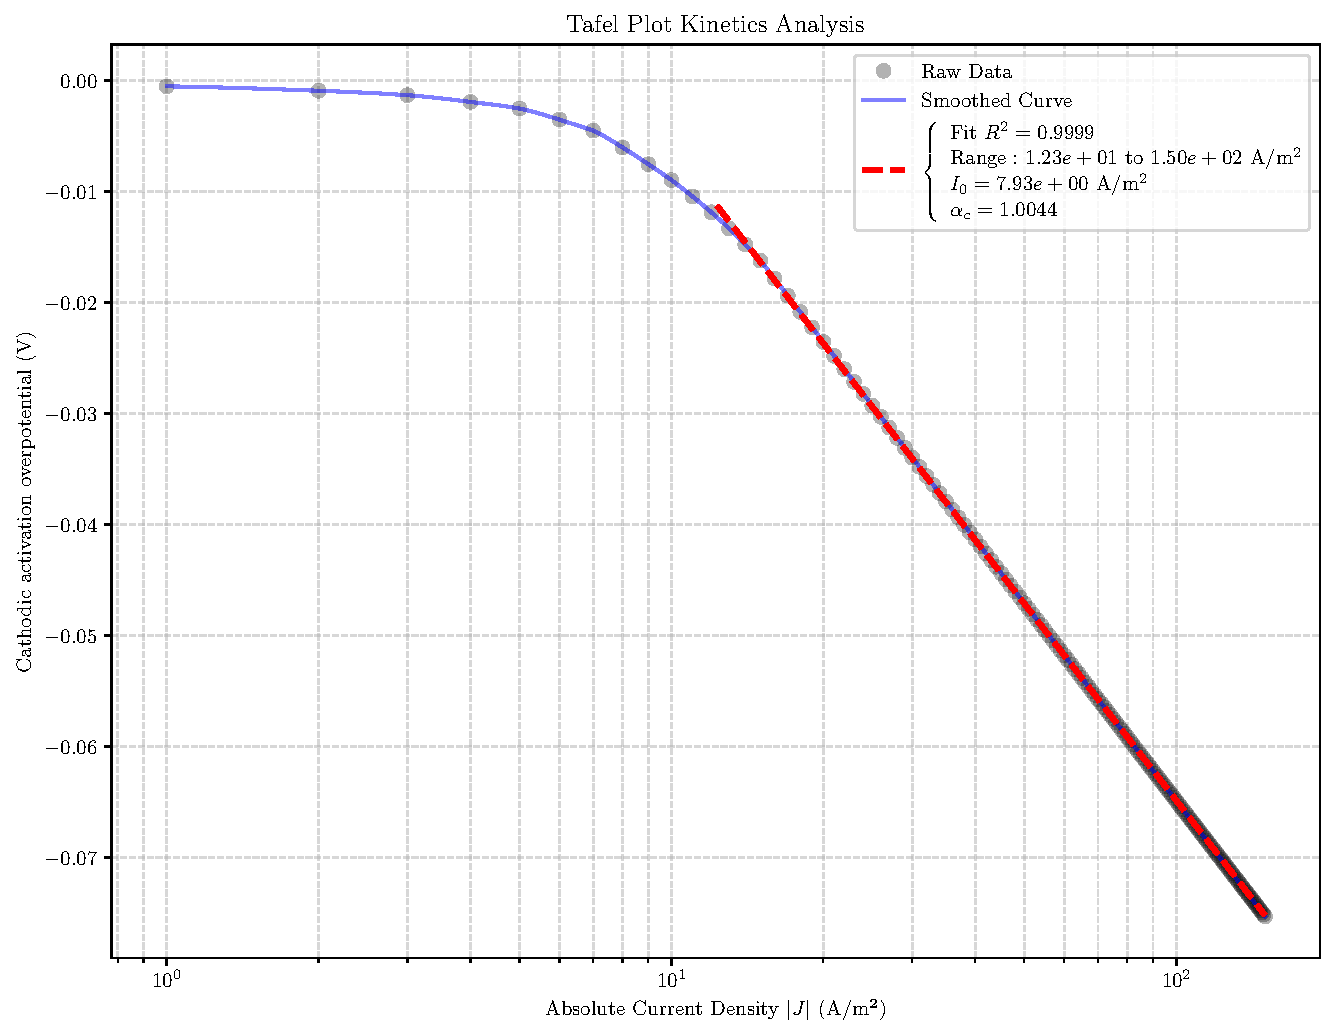
\includegraphics[height=\textheight, width=\textwidth, keepaspectratio]{tafel_analysis_output.pdf}
    \caption{Tafel Slope with fitted regression and parameter outputs.}
    \label{fig:Tafel}
\end{figure}

\section{Question 2}
$$
\eta_{ohmic}=j\cdot\frac{L}{\sigma}
$$
$$
\eta_{ohmic}=1\frac{A}{cm^2}\cdot\frac{0.01\text{ }cm}{0.1 \frac{S}{cm}}
$$
$$
\boxed{=0.1\text{ }V}
$$

\section{Question 3}
$$
ASR_{117} = \frac{L}{\sigma} = \frac{0.007\text{ }in\cdot2.54\frac{\text{ }cm}{in}}{0.05\frac{S}{cm}}=0.3556\text{ }\frac{\Omega}{cm^2}
$$
$$
ASR_{HP} = \frac{L}{\sigma} = \frac{0.02\text{ }mm\cdot0.1\frac{\text{ }cm}{mm}}{0.05\frac{S}{cm}}=0.04\text{ }\frac{\Omega}{cm^2}
$$
$$
\%_{decrease} = 100\cdot\left(1-\frac{Final}{Initial}\right)=1-\frac{0.04}{0.3556}\text{ }\boxed{=88.75\%}
$$
$$
\eta_{117} = J\cdot ASR = 1\frac{A}{cm^2}\cdot0.3556\text{ }\frac{\Omega}{cm^2} = 0.3556\text{ }V
$$
$$
\eta_{HP} = J\cdot ASR = 1\frac{A}{cm^2}\cdot0.04\text{ }\frac{\Omega}{cm^2} = 0.04\text{ }V
$$
$$
\eta_{117}-\eta_{HP} = 0.3556\text{ }V-0.04\text{ }V\text{ }\boxed{= 0.3156\text{ }V\text{ decrease}}
$$

\section{Question 4}
$$
\dot{n} = \frac{i}{nF},\quad where\quad n=2\text{ electron mole-eq's per mole H}_2\quad and\quad F=96485\text{ }C/mol
$$
$$
\dot{n} = \frac{1000\text{ }A}{2\text{ }mol\cdot 96485\text{ }C/mol} \text{ }\boxed{= 0.005\text{ }mol/s}
$$


\section{Code Availability}
The code used to generate the plot and fit is available in my 
GitHub repository: 

\noindent\url{https://github.com/Ben-JaminRees/Fuel-Cell-Course-Spring-2026}.

\end{document}